\begin{figure}[H]
  \centering
  % Primer grafo (G_1)
  \begin{minipage}[t]{0.49\textwidth}
    \centering
    \scalebox{0.7}{% Ajusta este valor (ej. 0.6, 0.7, 0.8) para controlar el tamaño
      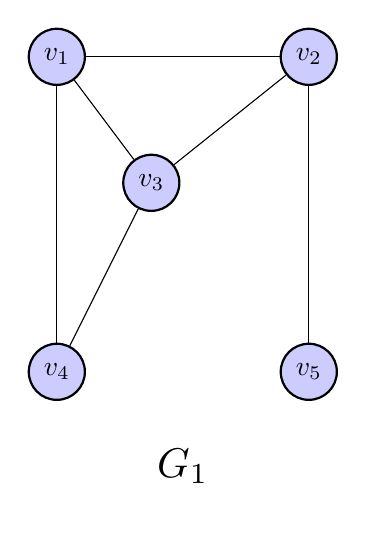
\begin{tikzpicture}[scale=.8,auto=left,every node/.style={circle,fill=blue!20,draw=black,thick}]
  % Vértices G1
  \node (n1) at (0, 4) {$v_1$};
  \node (n2) at (4, 4) {$v_2$};
  \node (n3) at (1.5, 2) {$v_3$};
  \node (n4) at (0, -1) {$v_4$};
  \node (n5) at (4, -1) {$v_5$};

  % Aristas G1 (Quitando n2/n4)
  \foreach \from/\to in {n1/n2, n1/n3, n1/n4, n2/n3, n2/n5, n3/n4}
    \draw (\from) -- (\to);

  % Título
  \node[draw=none, fill=none, scale=1.5] at (2, -2.5) {$G_1$};
\end{tikzpicture}

    }
  \end{minipage}%
  \hspace{-2em}%
  % Segundo grafo (G'_1)
  \begin{minipage}[t]{0.49\textwidth}
    \centering
    \scalebox{0.7}{% Usa el mismo factor de escala para que guarden proporción
      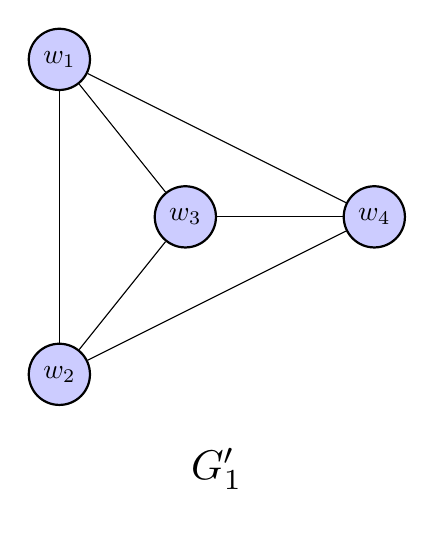
\begin{tikzpicture}[scale=.8,auto=left,every node/.style={circle,fill=blue!20,draw=black,thick}]
  % Vértices G'1
  \node (m1) at (0, 4) {$w_1$};
  \node (m2) at (0, -1) {$w_2$};
  \node (m3) at (2, 1.5) {$w_3$};
  \node (m4) at (5, 1.5) {$w_4$};

  % Aristas G'1
  \foreach \from/\to in {m1/m2, m1/m3, m1/m4, m2/m3, m2/m4, m3/m4}
    \draw (\from) -- (\to);

  % Título
  \node[draw=none, fill=none, scale=1.5] at (2.5, -2.5) {$G'_1$};
\end{tikzpicture}

    }
  \end{minipage}
  
  \caption{$\varphi$ es un homomorfismo de $G_1$ en $G'_1$}
  \label{fig:homomorfismo_grafos}
\end{figure}
